% Nama Kelompok : Linux
% Kelas : D4 TI 1A
% 1. Kadek Diva Krishna Murti (1174006)
% 2. Duvan Silalahi (1174011)
% 3. Oniwaldus (1174005)
% 4. Choirul Anam (1174004)
% 5. Sri Rahayu (1174015)
% 6. Ilham Habibi (1174028)



\begin{figure}[ht]
\centerline{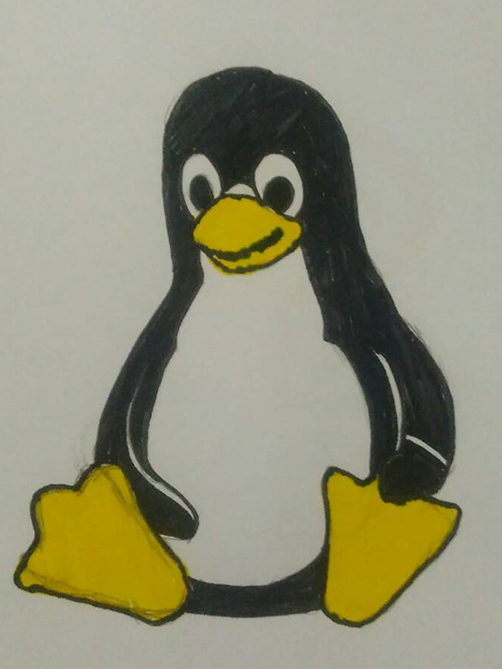
\includegraphics[width=0.5\textwidth]{figures/linux.jpg}}
\caption{Logo Linux.}
\label{Linux}
\end{figure}

Menurut Wahana Komputer dalam bukunya yang berjudul Mari Mengenal Linux menyebutkan bahwa Linux merupakan sebuah sistem operasi yang mirip dengan UNIX, dan merupakan implementasi independen dari sistem operasi POSIX, dengan ekstensi SYSV dan BSD sistem operasi UNIX, yang berjalan di mesin keluarga Intel 80386DX, atau yang lebih baru. Pada perkembangan berikutnya, Linux dapat berjalan di beberapa mesin lainnya seperti Sun Sparc, Mac, PowerPC, DEC Alpha, dan PPC mk86.\cite{komputer2005mari}

Linux adalah sistem operasi yang diedarkan secara gratis di bawah lisensi GNU General Public License (GPL), yang berarti source code Linux tersedia. Dengan begitu program tersebut dapat diubah, diadaptasi, maupun dikembangkan lebih lanjut oleh siapapun.

\section{Sejarah} 

Menurut Wahana Komputer dalam bukunya yang berjudul Mari Mengenal Linux menyebutkan bahwa dahulu Linux adalah proyek hobi yang dikerjakan oleh seorang mahasiswa Finlandia yang bernama Linus Torvalds. Dalam mengerjakan proyek hobinya tersebut, Linus Torvalds memperoleh inspirasi dari Minix, yaitu suatu sistem UNIX kecil yang dikembangkan oleh Andy Tanenbaum. Linux versi 0.01 dikerjakan sekitar bulan Agustus 1991. Kemudian pada tanggal 5 Oktober 1991 Linus Torvalds mengumumkan versi resmi dari Linux, yaitu 0.02. Versi ini hanya dapat menjalankan Bash (GNU Bourne Again Shell) dan gcc (GNU C Compiler). Meskipun Linux bukan merupakan sistem Unix resmi, namun Linux memiliki dasar warisan, budaya, arsitektur dan pengalaman sistem operasi Unix, sebuah sistem operasi yang sudah berjalan selama 28 tahun lebih. \cite{komputer2005mari}

\subsection{Pengenalan}

Menurut artikel Dasar-Dasar Linux menyebutkan bahwa Linus Torvalds membuat Kernel Linux, yaitu sebuah core Linux, di atas Minix dengan menggunakan bahasa C. Linux memiliki lisensi GNU, sebuah lisensi yang dikeluarkan untuk memungkinkan seseorang mendistribusikan, mengembangkan, dan memodifikasi source code suatu program secara gratis dan bebas. Pembuatan Linux di lakukan secara gotong royong oleh banyak programmer yang kebanyakan C/C++ Programmer di seluruh dunia via internet. Logo Linux adalah seekor penguin seperti gambar\ref{Linux}. Karena pada saat pengembangan Linux, Torvalds pernah di patuk oleh Penguin di sebuah kebun binatang yang menyebabkan dirinya demam dan dia bercita-cita agar orang lain dapat \"demam\" Linux. Nama Linux sendiri di adaptasi dari nama nya Linus. Saat ini, Linux memiliki beberapa Desktop Environment yang berbasis Grafis yaitu, KDE (K Desktop Environment) dan GNOME (GNU Network Object Model Environment). \cite{sofwan2003dasar}

\subsection{Aplikasi Yang Terdapat di Linux}

Menurut Wahana Komputer dalam bukunya yang berjudul Mari Mengenal Linux menyebutkan bahwa karena kernel Linux dikembangkan dengan usaha yang independent, banyak aplikasi yang tersedia, sebagai contoh, C Compiler menggunakan gcc dari Free Software Foundation GNU’s Project. Compiler ini banyak dipergunakan  pada lingkungan Hewlett-Packard dan Sun. Sekarang, banyak aplikasi Linux yang dapat dipergunakan untuk keperluan perkantoran seperti untuk spreadsheet, word processor, database dan Star Office yang merupakan program editor grafis yang memiliki tampilan dan fungsi layaknya Microsoft Office. Selain itu di Linux juga sudah tersedia versi Corel dan aplikasi seperti Matlab yang pada Linux dikenal sebagai Scilab. \cite{komputer2005mari}

Sekarang Linux merupakan sistem UNIX yang bisa digunakan untuk jaringan (networking), pengembangan software, bahkan untuk kebutuhan sehari-hari. Linux merupakan alternatif sistem operasi yang bisa didapatkan secara gratis jika dibandingkan dengan sistem operasi komersial lainnya dan dengan kemampuan yang setara atau bahkan lebih.


\section{Distribusi Linux}

Berikut ini beberapa distribusi (distro) Linux yang banyak peminatnya di Indonesia.

\begin{enumerate}

\item \textbf{Debian Linux}

\begin{figure}[ht]
\centerline{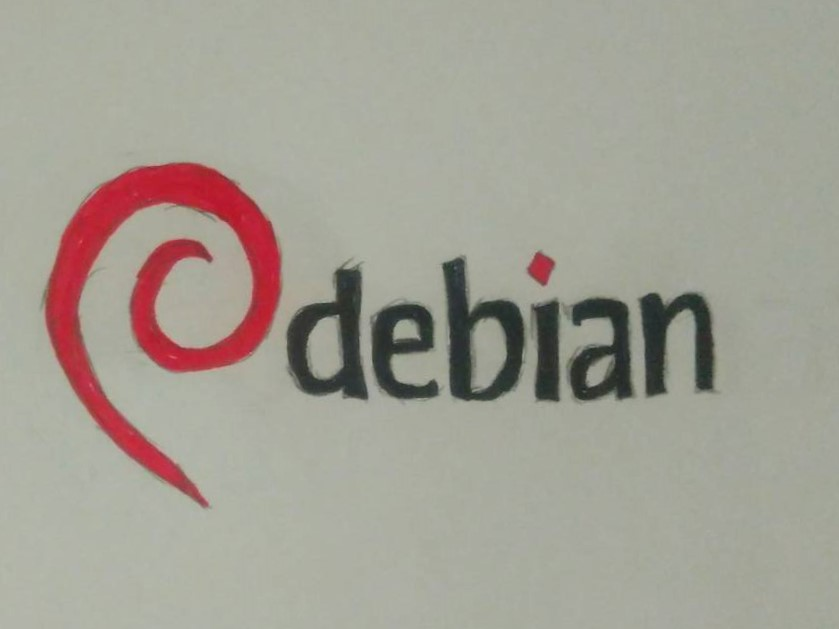
\includegraphics[width=0.4\textwidth]{figures/debian.jpg}}
\caption{Logo Debian Linux.}
\label{Debian}
\end{figure}

Menurut Wahana Komputer dalam bukunya yang berjudul Mari Mengenal Linux menyebutkan bahwa Debian merupakan distribusi dari Linux yang kurang terkenal, namun banyak penggunanya dari kalangan teknis. Mereka puas karena kestabilannya. Selain itu, format paket programnya yang menggunakan DEB dianggap lebih stabil daripada RPM menurut kalangan teknis.
Versi terakhir dari Debian adalah versi 2.1, yang dirilis pada tahun 1999. Dibandingkan dengan distribusi lainnya, Debian termasuk yang jarang dalam meng-update programnya. Debian juga sudah menggunakan metode autodetect untuk penggunaan peripheral pada komputer. \cite{komputer2005mari} Debian Linux memiliki logo seperti gambar \ref{Debian}.

Jika Anda ingin tahu lebih lanjut mengenai Debian Linux ataupun men-download programnya secara langsung, Anda bisa mengunjungi situsnya di http://www.debian.org

\textbf{\item RedHat Linux}


\begin{figure}[ht]
\centerline{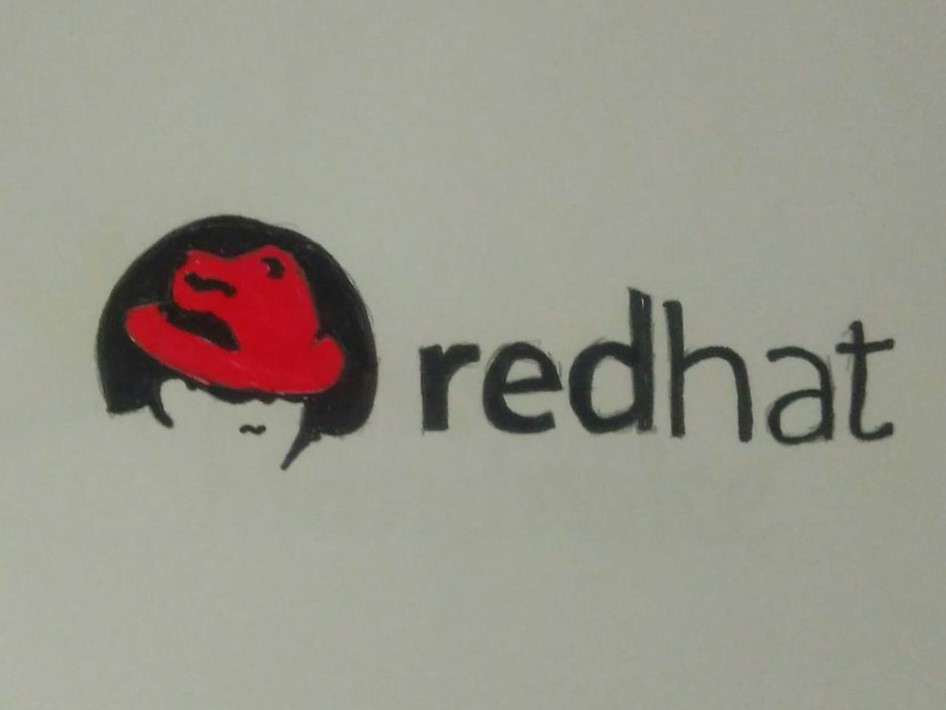
\includegraphics[width=0.4\textwidth]{figures/redhat.jpg}}
\caption{Logo RedHat Linux.}
\label{RedHat}
\end{figure}

Menurut Wahana Komputer dalam bukunya yang berjudul Mari Mengenal Linux menyebutkan bahwa  Redhat merupakan distribusi Linux yang paling popular di Indonesia dan Amerika yang dirancang khusus untuk server. RedHat di akui sebagai server tercepat dibandingkan dengan distribusi Linux lainnya untuk server. Selain dapat diguanakan sebagai server tercepat, RedHat juga dapat dipakai sebagai klien maupun digunakan sebagai desktop rumah tangga alias PC standlone. Saat ini Redhat sudah beredar dengan versi 6.2, menggunakan Standard Desktop Gnome.

Kelebihan lain dari RedHat adalah kemudahan dalam hal instalasinya. Ini merupakan revolusioner Linux. Ketika distribusi linux lainnya membuat penggunanya awalnya menjadi putus asa pada saat prosedur instalasinya, RedHat hadir dengan prosedur instalasi yang termudah pada masanya.
Hal revolusioner lainnya adalah RedHat membuat format paket program RPM menjadi standar baku file biner pada Linux, yang kemudian digunakan oleh distribusi lainnya seperti SuSE, Mandrake dan Caldera. \cite{komputer2005mari} Redhat Linux memiliki logo seperti gambar \ref{RedHat}.

Jika Anda ingin tahu lebih lanjut mengenai RedHat Linux ataupun men-download programnya secara langsung, Anda bisa mengunjungi situsnya di http://www.redhat.com

\textbf{\item Mandrake Linux}


\begin{figure}[ht]
\centerline{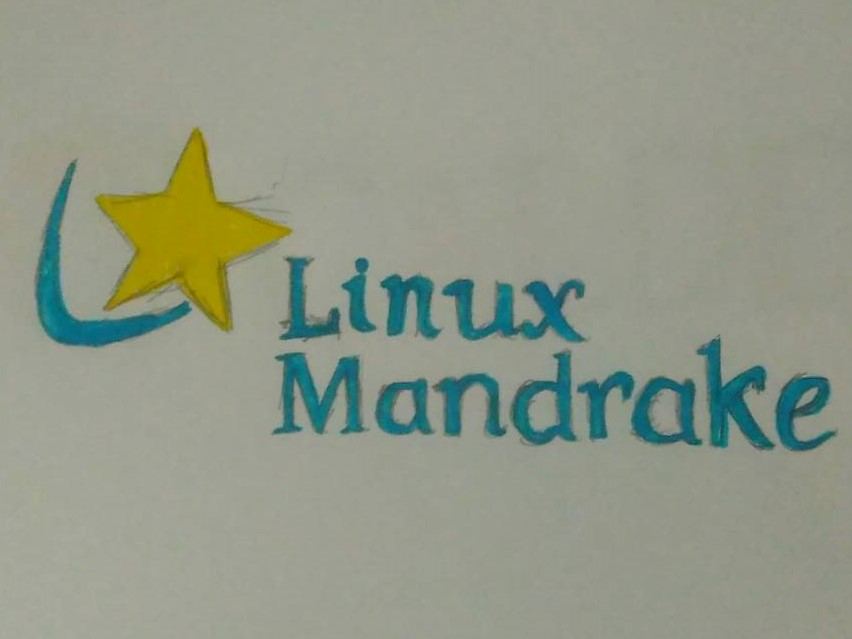
\includegraphics[width=0.4\textwidth]{figures/mandrake.jpg}}
\caption{Logo Mandrake Linux.}
\label{Mandrake}
\end{figure}

Menurut Wahana Komputer dalam bukunya yang berjudul Mari Mengenal Linux menyebutkan bahwa Mandrake adalah saudara muda dari RedHat, karena keduanya dibuat oleh satu distribusi. Bila RedHat direkomendikasikan sebagai server, maka Mandrake direkomendasikan oleh pembuat distro RedHat sebagai klien yang handal, namun diutamakan yang menggunakan prosesor Pentium. Meskipun demikian, tidak menutup kemungkinan penggunaan Mandrake sebagai server yang handal juga.

Tujuan diciptakannya Mandrake pada awalnya adalah untuk mempermudah penggunanya dalam melakukan instalasi dan penggunaan Linux. Sebelum diluncurkannya Corel Linux, Mandrake merupakan salah satu distribusi Linux yang paling populer. Jika RedHat keluar dengan desktop manager menggunakan Gnome, maka Mandrake keluar dengan desktop manager KDE buatan SuSE Jerman. Saat ini Mandrake sudah keluar dengan versi 7.1. \cite{komputer2005mari} Mandrake Linux memiliki logo seperti gambar \ref{Mandrake}.

Jika Anda ingin tahu lebih lanjut mengenai Mandrake Linux ataupun men-download programnya secara langsung, Anda bisa mengunjungi situsnya di http://www.linux-mandrake.com

\textbf{\item Caldera Open Linux}


\begin{figure}[ht]
\centerline{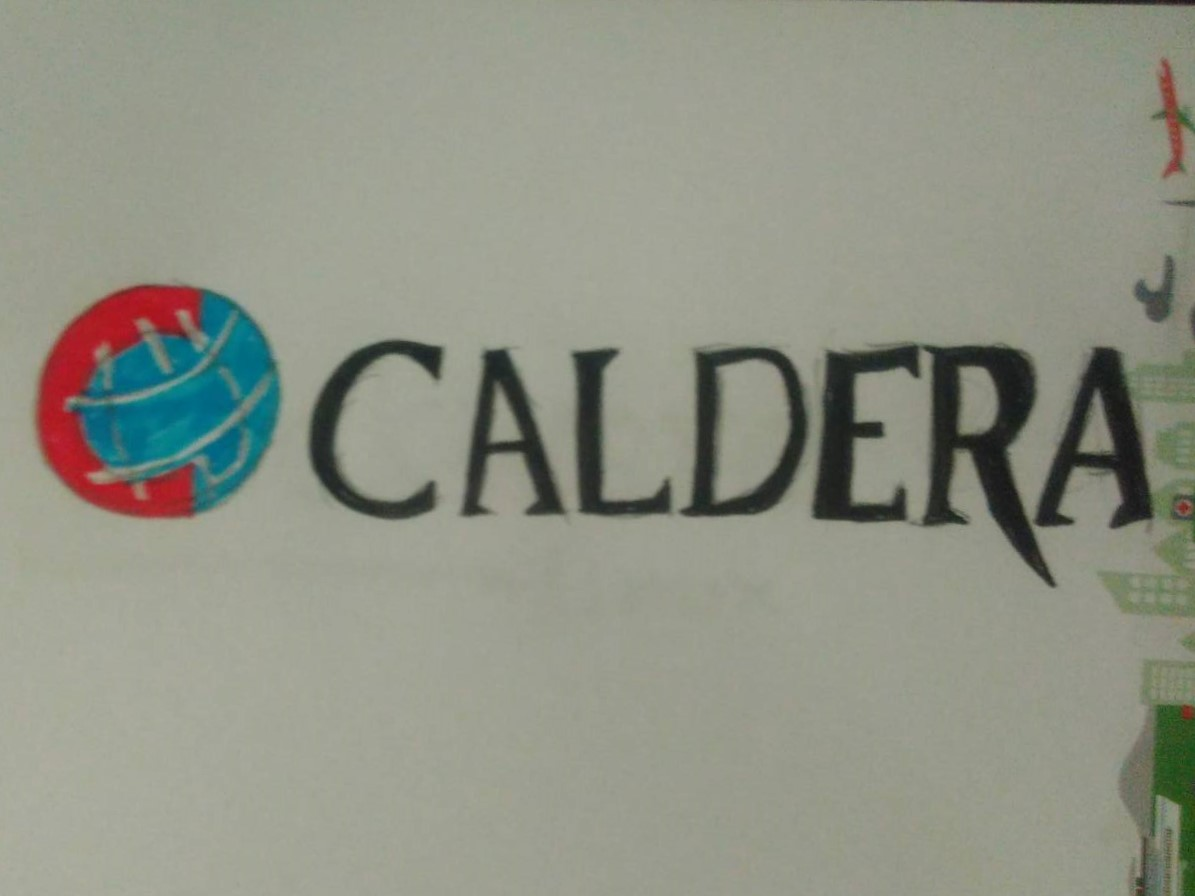
\includegraphics[width=0.4\textwidth]{figures/caldera.jpg}}
\caption{Logo Caldera Open Linux.}
\label{Caldera}
\end{figure}

Menurut Wahana Komputer dalam bukunya yang berjudul Mari Mengenal Linux menyebutkan bahwa Caldera merupakan merupakan distribusi Linux yang dirancang untuk mempermudah pemakainya dalam pengoperasiannya. Caldera sendiri dirancang sebagai distribusi Linux yang keselurahannya dalam bentuk grafis. Sejak mulai instalasi hingga setting hardware, semuanya dalam bentuk grafis. Yang mengagumkan adalah pada saat melakukan instalasi Caldera, Anda akan disuguhi game tetris untuk mengisi waktu, sembari menunggu transfer program. Selain itu Caldera merupakan distribusi Linux pertama yang menggunakan auto-detect hardware (seperti plug dan  play pada Mac). \cite{komputer2005mari} Caldera Linux memiliki logo seperti gambar \ref{Caldera}.

Jika Anda ingin tahu lebih lanjut mengenai Caldera Open Linux ataupun men-download programnya secara langsung, Anda bisa mengunjungi situsnya di http://www.caldera-system.com

\textbf{\item Slackware Linux}


\begin{figure}[ht]
\centerline{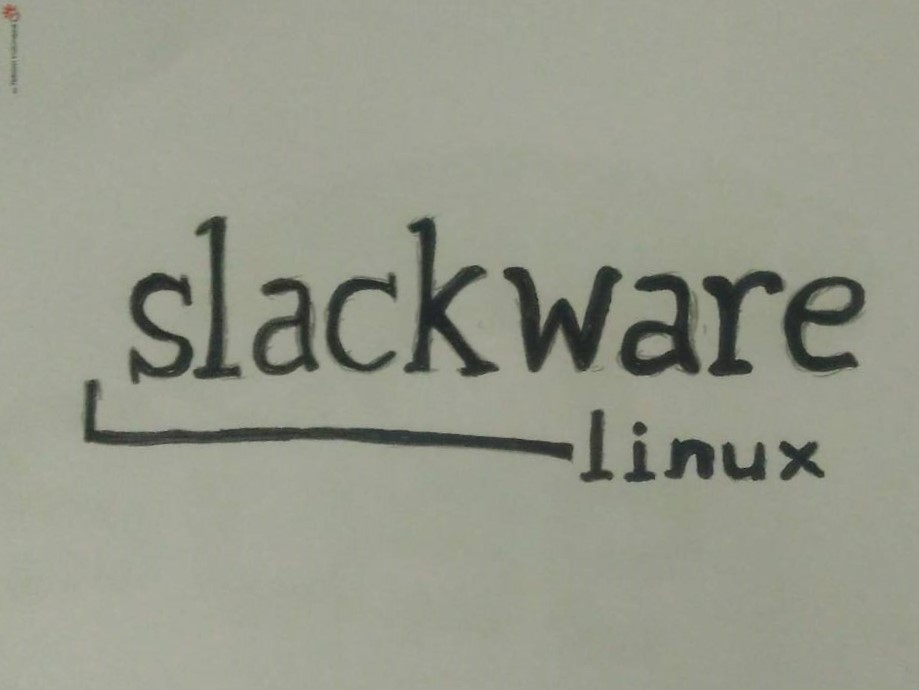
\includegraphics[width=0.4\textwidth]{figures/slackware.jpg}}
\caption{Logo Slackware Linux.}
\label{Slackware}
\end{figure}

Menurut Wahana Komputer dalam bukunya yang berjudul Mari Mengenal Linux menyebutkan bahwa Slackware dibuat oleh Patrick Volkerding, Slackware merupakan distribusi Linux yang pertama, dengan tampilan yang sederhana tapi penggunaannya manual tidak seperti produk Linux yang lain. Biasanya Slackware digunakan oleh pengguna Linux yang sudah pro atau bisa juga yang ingin menjadi pengguna Linux yang pro. Slackware awalnya turunan dari Softlanding Linux System dan merupakan yang paling populer dari distribusi Linux asli. Versi Slackware Linux yang pertama tersedia di publik adalah versi 1.0 yang rilis pada 16 juli 1993. Slackware Linux mengacu pada prinsip KISS (Keep It Simple Stupid). \cite{ komputer2005mari}. Slackware Linux memiliki logo seperti gambar \ref{Slackware}.

Jika Anda ingin tahu lebih lanjut mengenai Slackware Linux ataupun men-download programnya secara langsung, Anda bisa mengunjungi situsnya di http://www.slackware.com

\textbf{\item Suse Linux}


\begin{figure}[ht]
\centerline{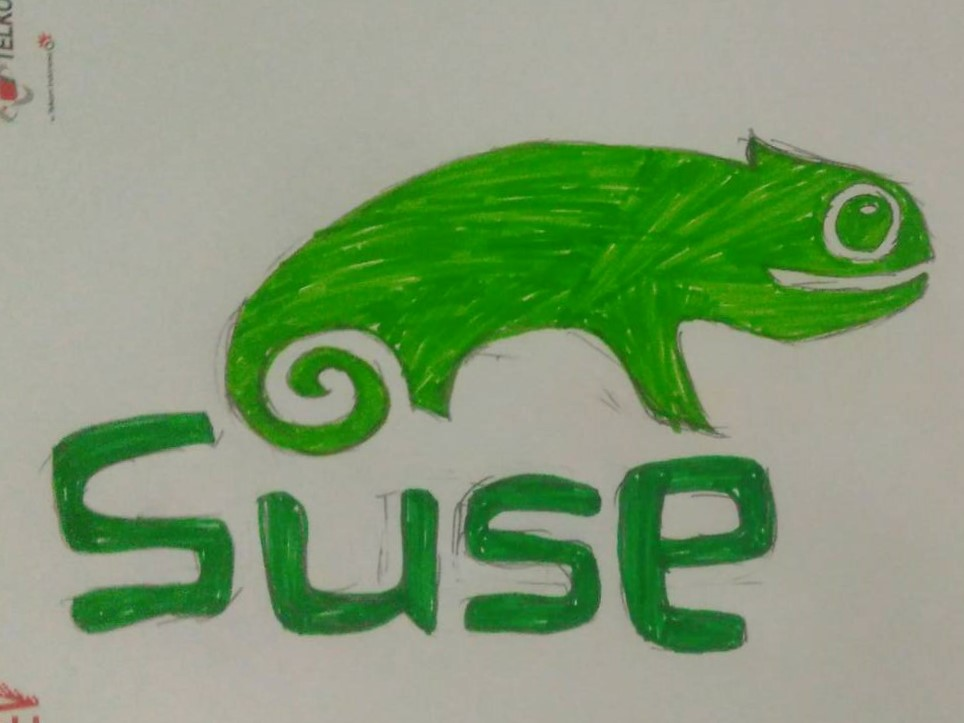
\includegraphics[width=0.4\textwidth]{figures/suse.jpg}}
\caption{Logo Suse Linux.}
\label{Suse}
\end{figure}

Menurut Wahana Komputer dalam bukunya yang berjudul Mari Mengenal Linux menyebutkan bahwa Suse Linux merupakan distribusi Linux yang sistemnya dioperasikan di atas kernel. Suse Linux merupakan produk Linux yang sangat populer di Negara Eropa. Dilengkapi dengan KDE dan central setting YaST (Yet Another Settup Tools) yang digunakan sebagai sistem operasi untuk deskop dan server. Suse bermula pada tahun 1990-an yang didirikan oleh perusahaan Novell yang dimana Linux terdiri dari 50 keping disket dan dapat di unduh atau diambil lewat internet. Ada 2 macam jenis Suse Linux yaitu, Suse Linux Enterprise dan Open Suse. Suse Linux Enterprise terdiri dari 2 paket yaitu, Suse Linux Enterprise Server dan Suse Linux Enterprise Deskop. Open Suse merupakan sebuah proyek masyarakat yang disponsori oleh Novell dan dirancang untuk pengguna rumah. \cite{komputer2005mari} Suse Linux memiliki logo seperti gambar \ref{Suse}.

Jika Anda ingin tahu lebih lanjut mengenai Suse Linux ataupun men-download programnya secara langsung, Anda bisa mengunjungi situsnya di http://www.suse.com

\textbf{\item Corel Linux}


\begin{figure}[ht]
\centerline{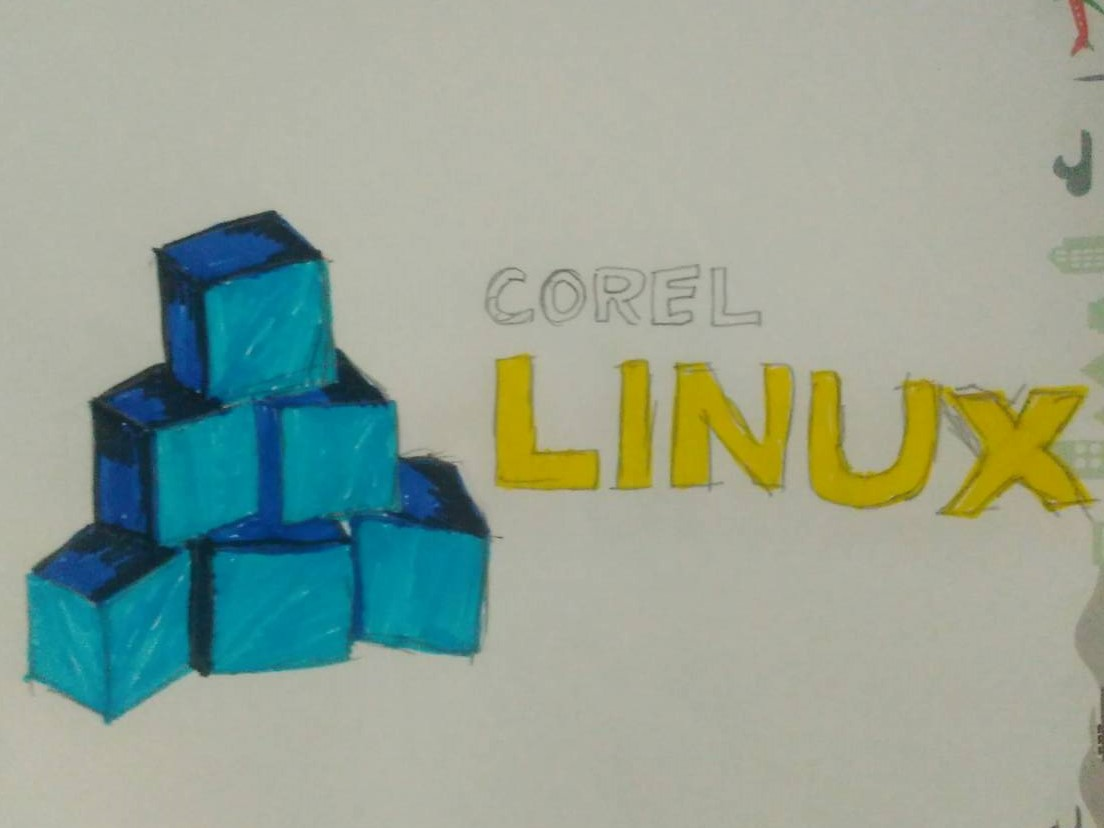
\includegraphics[width=0.4\textwidth]{figures/corel.jpg}}
\caption{Logo Corel Linux.}
\label{Corel}
\end{figure}

Menurut Wahana Komputer dalam bukunya yang berjudul Mari Mengenal Linux menyebutkan bahwa Corel Linux dibuat oleh distribusi Linux yaitu Debian. Corel Linux mendukung operasi sistem open source dibawah naungan GNU. Harganya juga sangat terjangkau dan dapat langsung di instal dengan sistem operasi lain dan juga bisa tanpa sistem operasi lain. Corel Linux juga bisa dinstal pada partisi dan file sistem Windows yang menjadikan corel linux seolah-olah adalah program aplikasi Windows. Corel Linux dirancang sebagai End-User. Pada Corel Linux semuanya serba grafis, dimulai saat instalasi sampai pada boot sistem. Pada Corel Linux kita tidak akan menjumpai baris teks seperti pada Linux yang lain, atau bahkan seperti pada Windows yang masih kelihatan baris teks. Semua sistem Corel Linux ini sangat sederhana sampai pada setting jaringannya lebih sederhana daripada Windows. \cite{komputer2005mari} Corel Linux memiliki logo seperti gambar \ref{Corel}.

Jika Anda ingin tahu lebih lanjut mengenai Corel Linux ataupun men-download programnya secara langsung, Anda bisa mengunjungi situsnya di http://www.linux.corel.com

\textbf{ \item Turbo Linux}


\begin{figure}[ht]
\centerline{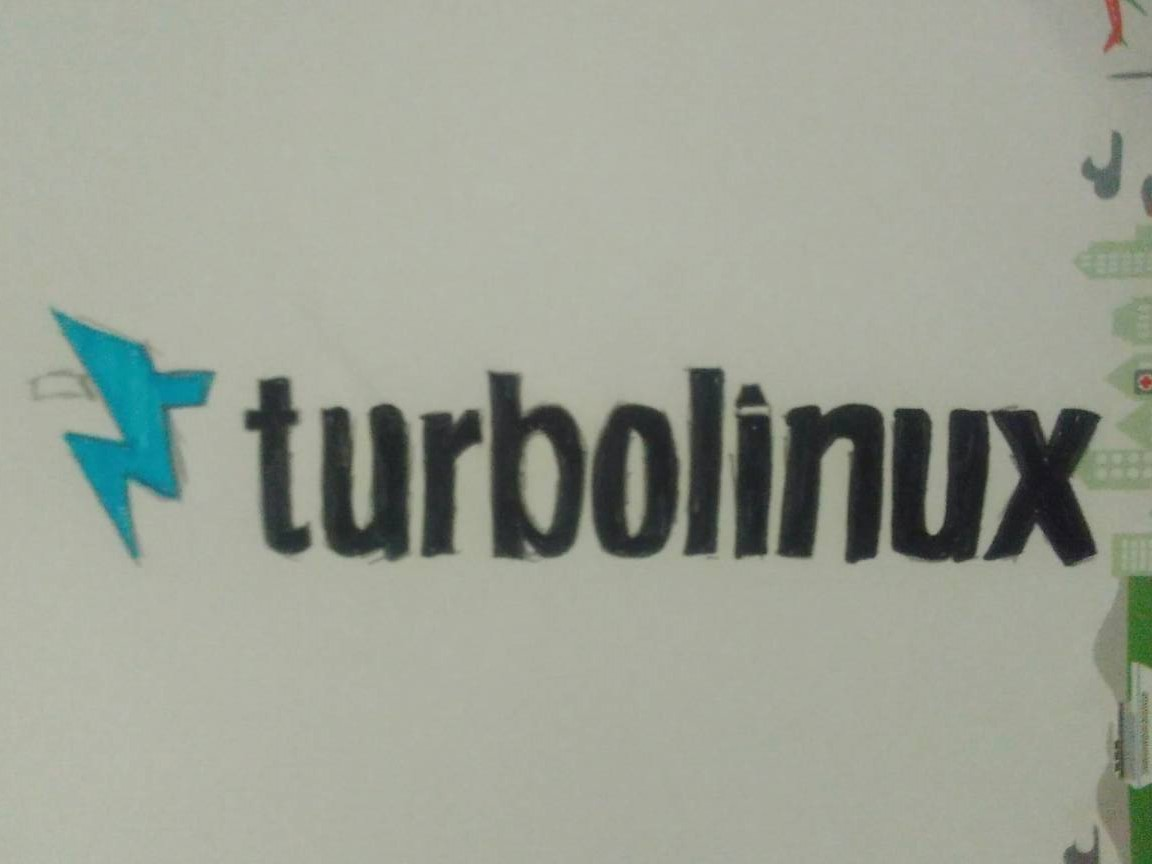
\includegraphics[width=0.4\textwidth]{figures/turbo.jpg}}
\caption{Logo Turbo Linux.}
\label{Turbo}
\end{figure}

Menurut Wahana Komputer dalam bukunya yang berjudul Mari Mengenal Linux menyebutkan bahwa Turbo Linux sangat populer dan terkenal di Asia. Turbo Linux menduduki posisi pertama pada Linux pilihan. Turbo Linux diciptakan dari berbagai program-program under Linux atau UNIX. Turbo Linux mendesain produknya dengan menggabungkan beberapa kelebihan dari open source dan dari perangkat lunak komersial. Turbo Linux menyertakan Cross Platform Management Software dalam produk-produk work station server dan clustering yang memungkinkan kemudahan dalam memanage networks dan sistem. Ada beberapa fitur Turbo Linux yaitu, Kernel 2.4.5, Glibc 2.2.3, Gcc 2.95.3, Xfree86 4.1.10, Rpm 4.0.2, Kde 2.1.2, Gnome 1.4. \cite{komputer2005mari} Turbo Linux memiliki logo seperti gambar \ref{Turbo}.

Jika Anda ingin tahu lebih lanjut mengenai Turbo Linux ataupun men-download programnya secara langsung, Anda bisa mengunjungi situsnya di http://www.turbo-linux.com



\end{enumerate}

\section{Kelebihan Linux}

Berikut ini beberapa kelebihan dari penggunaan Sistem Operasi Linux, di antaranya adalah:

\begin{itemize}

\item Merupakan salah satu sistem operasi yang bersifat open source, yang berarti penggunanya dapat melihat maupun mengubah source codenya tanpa terkena sanksi.

\item Merupakan salah satu sistem operasi yang freeware di bawah lisensi GNU, yang berarti penggunanya tidak harus mengeluarkan biaya untuk memiliki sistem operasi ini.

\item Tidak memerlukan spesifikasi hardware yang tinggi untuk menjalankan sistem operasi ini.

\item Linux kebal  terhadap virus karena Linux mendukung adanya file permissions (ijin file), yang dapat mencegah perubahan atau penghapusan file tanpa ijin dari pemiliknya.

\item Lebih dari satu orang dapat menggunakan program yang sama atau berbeda dari satu mesin yang sama, pada saat bersamaan, di terminal yang sama atau berbeda.

\item Dalam satu komputer, pengguna dapat melakukan login dengan nama user yang sama atau berbeda lebih dari satu kali, tanpa perlu menutup sesi sebelumnya.

\item Mengeksekusi suatu program dan mengakses data dapat dilakukan secara bersama-sama tanpa harus khawatir terjadi hang atau stack.

\item Dalam penggunaannya Linux sangat stabil sehingga bisa mengcopy, mengedit, menghapus satu file atau data secara bersamaan pada saat data atau file tersebut dieksekusi.

\item Jumlah login user atau operator yang dimiliki tidak terbatas sehingga user bisa mencapai 254 klien secara bersamaan dan dilengkapi dengan password.

\item Linux dapat digunakan sebagai Web Server atau sebagai FTP Server.

\item Linux mendukung fasilitas GUI (Graphic User Interface).

\end{itemize}

\section{Kelemahan Linux}

Berikut ini beberapa kelemahan dari penggunaan Sistem Operasi Linux, di antaranya adalah:

\begin{itemize}

\item Cara penggunaanya sangat berbeda sekali dengan sistem operasi lainnya seperti Windows sehingga perlu waktu dan tenaga ekstra untuk mempelajari penggunaanya. Apalagi bagi yang baru belajar komputer akan mengalami kesulitan dalam penggunaannya.

\item Banyak aplikasi-aplikasi yang belum mendukung penggunaanya dalam Linux.

\item Tidak dapat mendukung beberapa hardware-hardware tertentu.

\item Sedikit penggunanya, hal ini menyebabkan sedikit juga orang-orang yang dapat di jadikan ajang bertanya sesama pengguna Linux.

\end{itemize}

\subsection{Pengertian DOS dan UNIX/Linux}
DOS (Disk Operating System) adalah sebuanh system operasi yang digunakan di komputer pribadi, dimana DOS Sendiri merupakan buatan perusahaan microsoft. Namun berbeda dengan Windows system operasi DOS tidak bersifat multi-tasking (dapat menjalankan aplikasi/proses berdasarkan system pembagian waktu/time).
UNIX/Linux merupakan perangkat lunak computer yang mengendalikan operasi dasar, system computer unix terdiri dari jumlah program yang dirancang untuk mengontrol interaksi antara fungsi-fungsi pada mesin berasas rendah dengan program aplikasi.
\subsection{Perintah-Perintah DOS dan UNIX}
DOS	UNIX
ATTRIB (+-)
BACKUP	Chmode (mode) file
Tar -Mcvf
CD	Cd
COPY	Cp
DEL	Rm
DIR	Is, dir
MD	Mkdir
EDIT	Vi, joe, pico, jstar
FORMAT	Fdformat, mkfs
Mount, unmount
HELP	Man [command]
Info [command]
REN	Rv
RESTORE	Tar –xvf
TYPE	Cat, more, less
WIN	Startx
PRINT	Lpt
PRN	/dev/lp0. /dev/lp1
NUL	/dev/null
